\chapter{Big-Line-Big-Clique conjecture} A conjectura seguinte foi proposta por \cite{visibilitygraph}:
\begin{conjectura}\label{conj1}
    Dados dois inteiros $k,l\geq2$, existe um $n=n(k,l)$ tal que todo conjunto finito $P$ com pelo menos $n$ pontos no plano contém ou $k$ pontos visíveis entre si (alternativamente, $\mathcal V(P)$ possui uma $k$-clique) ou $l$ pontos colineares.
\end{conjectura}
Embora seu enunciado seja simples, poucos resultados foram encontrados para ela, ainda estando em aberto para valores de $k$ e $l$ a partir de $6$ e $4$ respectivamente.

Para nos habituarmos com o problema, vamos começar pelos casos mais básicos:

\section{Casos triviais}
Primeiramente, se $k=2$ (ou $l=2$), com certeza todo conjunto com pelo menos dois pontos tem dois pontos visíveis (e dois pontos colineares).

Se $k=3$, ou se tem três pontos visíveis ou todos os pontos no conjunto são colineares, então $n(3,l)=max\{3,l\}$.

Se $l=3$, ou todos os pontos são visíveis para todos os outros ou algum ponto não deixa outros dois se verem, se tendo três pontos colineares. $n(k,3) = max\{k,3\}$.


\section{Caso $k=4$}
Vamos mostrar que os conjuntos que não possuem quatro pontos visíveis possuem muitos pontos colineares. Isto é, para todo $l$ existe um $n$ tal que todo conjunto $P$ com pelo menos $n$ pontos que não possui quatro pontos visíveis possui pelo menos $l$ pontos colineares.

Como visto no teorema \ref{planork4} do capítulo anterior, um conjunto que não possui quatro pontos visíveis possui grafo de visibilidade plano. Vamos usar o seguinte lema que caracteriza os grafos de visibilidade planos:

\begin{figure}
    \begin{tikzpicture}
        \node(A) {$(a)$};
        \node[draw, shape=circle] (A1) [right = 0.3cm of A] {};
        \node[draw, shape=circle] (A2) [right = 0.6cm of A1] {};
        \node[draw, shape=circle] (A3) [right = 0.6cm of A2] {};
        \node[draw, shape=circle] (A4) [right = 0.6cm of A3] {};
        \node[draw, shape=circle] (A5) [right = 0.6cm of A4] {};
        \draw (A1)--(A2);
        \draw (A2)--(A3);
        \draw (A3)--(A4);
        \draw (A4)--(A5);

        \node(B) [below = 1.2cm of A] {$(b)$};
        \node[draw, shape=circle] (B1) [right = 0.3cm of B] {};
        \node[draw, shape=circle] (B2) [right = 0.6cm of B1] {};
        \node[draw, shape=circle] (B3) [right = 0.6cm of B2] {};
        \node[draw, shape=circle] (B4) [right = 0.6cm of B3] {};
        \node[draw, shape=circle] (B5) [right = 0.6cm of B4] {};
        \node[draw, shape=circle] (B6) [above = 0.6cm of B3] {};
        \draw (B1)--(B2);
        \draw (B2)--(B3);
        \draw (B3)--(B4);
        \draw (B4)--(B5);
        \draw (B1)--(B6);
        \draw (B2)--(B6);
        \draw (B3)--(B6);
        \draw (B4)--(B6);
        \draw (B5)--(B6);

        \node(C) [below = 1.2cm of B] {$(c)$};
        \node[draw, shape=circle] (C1) [right = 0.3cm of C] {};
        \node[draw, shape=circle] (C2) [right = 0.6cm of C1] {};
        \node[draw, shape=circle] (C3) [right = 0.6cm of C2] {};
        \node[draw, shape=circle] (C4) [right = 0.6cm of C3] {};
        \node[draw, shape=circle] (C5) [right = 0.6cm of C4] {};
        \node[draw, shape=circle] (C6) [above = 0.6cm of C3] {};
        \node[draw, shape=circle] (C7) [below = 0.6cm of C3] {};
        \draw (C1)--(C2);
        \draw (C2)--(C3);
        \draw (C3)--(C4);
        \draw (C4)--(C5);
        \draw (C1)--(C6);
        \draw (C2)--(C6);
        \draw (C3)--(C6);
        \draw (C4)--(C6);
        \draw (C5)--(C6);
        \draw (C1)--(C7);
        \draw (C2)--(C7);
        \draw (C3)--(C7);
        \draw (C4)--(C7);
        \draw (C5)--(C7);

        \node(D) [right = 5.4cm of A] {$(d)$};
        \node (D') [right = 0.3cm of D] {};
        \node[draw, shape=circle] (D1) [right = 0.3cm of D'] {};
        \node[draw, shape=circle] (D2) [right = 0.6cm of D1] {};
        \node[draw, shape=circle] (D3) [right = 0.6cm of D2] {};
        \node[draw, shape=circle] (D4) [right = 0.6cm of D3] {};
        \node[draw, shape=circle] (D5) [right = 0.6cm of D4] {};
        \node[draw, shape=circle] (D6) [above = 0.6cm of D'] {};
        \node[draw, shape=circle] (D7) [below = 0.6cm of D'] {};
        \draw (D1)--(D2);
        \draw (D2)--(D3);
        \draw (D3)--(D4);
        \draw (D4)--(D5);
        \draw (D1)--(D6);
        \draw (D2)--(D6);
        \draw (D3)--(D6);
        \draw (D4)--(D6);
        \draw (D5)--(D6);
        \draw (D1)--(D7);
        \draw (D2)--(D7);
        \draw (D3)--(D7);
        \draw (D4)--(D7);
        \draw (D5)--(D7);
        \draw (D6)--(D7);

        \node(E) [below =2.4cm of D] {$(e)$};
        \node[draw, shape=circle] (E1) [below right = 1cm and 0.3cm of E] {};
        \node[draw, shape=circle] (E2) [right = 3cm of E1] {};
        \node[draw, shape=circle] (E3) [above right = 2.8cm and 1.5cm of E1] {};
        \node[draw, shape=circle] (E4) [below left = 1.1cm and 0cm of E3] {};
        \node[draw, shape=circle] (E5) [below left = 0.9cm and 0cm of E4] {};
        \node[draw, shape=circle] (E6) [below right = 0.5cm and 0.55cm of E4] {};
        \draw (E1)--(E2);
        \draw (E2)--(E3);
        \draw (E3)--(E1);
        \draw (E1)--(E4);
        \draw (E1)--(E5);
        \draw (E2)--(E5);
        \draw (E2)--(E6);
        \draw (E3)--(E6);
        \draw (E3)--(E4);
        \draw (E4)--(E5);
        \draw (E5)--(E6);
        \draw (E6)--(E4);
    \end{tikzpicture}
    \caption{Tipos de grafos de visibilidade planos}
    \label{fig:visibilidadeplanar}
\end{figure}

\begin{lema}[\cite{planar}]\label{visibilidadeplanar}
    Seja $P$ um conjunto finito de pontos no plano. Então $\mathcal V(P)$ é plano se e somente se satisfaz uma das condições:
    \begin{enumerate}[label=(\alph*)]
        \item
            Todos os pontos de $P$ são colineares.
        \item
            Todos os pontos de $P$ são colineares exceto um.
        \item
            Todos os pontos de $P$ são colineares exceto dois pontos não visíveis.
        \item
            Todos os pontos de $P$ são colieares exceto dois pontos $p$ e $q$ tais que o segmento $\overline{pq}$ não intercepta o menor segmento que contém $P\setminus\{p,q\}$
        \item
            $\mathcal V(P)$ é o grafo $(e)$ desenhado na figura \ref{fig:visibilidadeplanar}
    \end{enumerate}
\end{lema}
\begin{proof}
    Como pode ser visto na figura \ref{fig:visibilidadeplanar} e pode ser facilmente demonstrado, se um grafo de visibilidade satisfaz alguma das condições $(a)-(e)$, ele é plano. Para mostrar a outra direção, seja $P$ um conjunto finito de pontos no plano tal que $\mathcal V(P)$ é plano.

    Se $P$ contém no máximo dois pontos, $P$ satisfaz $(a)$. Então vamos supor que $|P|\geq 3$. Seja $L$ um maior conjunto de pontos colineares em $P$ e $\hat L$ a reta que contém $L$. $|L|\geq 2$. Se $|L|=2$, então $L$ satisfaz $(a)$, $(b)$ ou $(e)$. Vamos supor então que $|L|\geq3$.

    A reta $\hat L$ divide o plano em dois semiplanos. Sejam $S$ e $T$ os conjuntos de vértices em cada um desses semiplanos tal que $|S|\geq|T|$. Se $|S|$ for no máximo 1, então $P$ satisfaz algum de $(a)-(d)$. Então supor que $|S|\geq2$. Seja $v$ um ponto de $S$ mais próximo de $\hat L$ e seja $w$ um ponto de $S\setminus\{v\}$ mais próximo de $\hat L$. Note que a reta que contém $v$ e $w$ não é paralela a $\hat L$, pois, se fosse, para todos $x,y\in L$, as arestas $\overline{vx}$ e $\overline{wy}$ ou as arestas $\overline{vy}$ e $\overline{wx}$ se interceptariam e, como o grafo é plano, existiria um vértice nessa interseção que seria mais próximo de $\hat L$ do que $v$, contradizendo a escolha de $v$. Então a reta que contém $v$ e $w$ intercepta $\hat L$ em um ponto, digamos, $p$.

    Vamos mostrar que em $\hat L$ se tem no máximo um vértice de cada lado de $p$. Para isso, suponha que existam dois vértices $x,y\in L$ tais que $x$ esteja entre $y$ e $p$. Então as arestas $\overline{vy}$ e $\overline{wx}$ se interceptam num ponto mais próximo de $\hat L$ do que $v$ e, como o grafo é plano, deve existir um vértice nessa interseção, contradizendo a escolha de $v$. Mas como $|L|\geq3$, $L$ tem que possuir exatamente $3$ pontos: $p$ e um ponto de cada lado de $p$, que vamos chamar de $x$ e $y$.

    Agora vamos mostrar que $S=\{v,w\}$. Suponha que $S$ contém um terceiro ponto $u$. $u$ não está na mesma reta que $p$, $v$ e $w$ pois $L$ tem tamanho máximo. Pela escolha de $v$ e $w$, $u$ está mais longe de $\hat L$ do que $w$. Então $\overline{uv}$ intercepta $\overline{wx}$ ou $\overline{wy}$ num ponto mais próximo de $\hat L$ do que $w$, contradizendo a escolha de $w$. Logo $|S|=2$. Então $|T|\leq2$.

    Se $T=\emptyset$, então $P$ satisfaz $(c)$. Suponha que $T\neq\emptyset$. Seja $u$ um ponto de $T$ e $q$ a interseção da reta que contém $u$ e $v$ e da reta $\hat L$. Suponha que $q$ não seja um vértice de $L$. Se $q$ está entre $x$ e $y$, então as arestas $\overline{vu}$ e $\overline{px}$ ou $\overline{py}$ se interceptam em $q$, e como o grafo é plano, $q$ tem que ser um vértice do grafo, o que é uma contradição. Similarmente, se $q$ não está entre $x$ e $y$, as arestas $\overline{uv}$ e $\overline{wx}$ ou $\overline{wy}$ se interceptam no ponto $q$, gerando uma contradição. Então $u$ intercepta $\hat L$ num vértice. Esse vértice não pode ser $p$, pois se fosse isso contradiria a escolha de $L$.

    Suponha que existam dois pontos $u_1$ e $u_2$ em $T$. Se $u_1$ está na mesma reta que $v$ e $x$ e $u_2$ está na mesma reta que $v$ e $y$. As arestas $\overline{u_1y}$ e $\overline{u_2x}$ se interceptam em um ponto de $T$ que não está na mesma reta que $v$ e $x$ nem que $v$ e $y$, o que é uma contradição. Se $u_1$ e $u_2$ estão na mesma reta que $v$ e $x$, suponha sem perda de generalidade que $u_1$ está entre $x$ e $u_2$, então as arestas $\overline{u_1y}$ e $\overline{u_2x}$ se interceptam em um ponto de $T$ que não está na mesma reta que $v$ e $x$ nem que $v$ e $y$, o que é uma contradição. Do mesmo jeito, se $u_1$ e $u_2$ estão na mesma reta que $v$ e $y$ também temos uma contradição. Portanto $|T|=1$. Sem perda de generalidade, digamos que $u$ é colinear com $v$ e $x$. Assim $\{p,u,v,x,y,w\}$ forma o grafo $(e)$ da figura \ref{fig:visibilidadeplanar}
\end{proof}
\begin{teorema}
    Seja $P$ um conjunto finito de pontos no plano. As seguintes afirmações são equivalentes:
    \begin{itemize}
        \item
            $P$ satisfaz $(a)$, $(b)$, $(c)$ ou $(e)$ do lema \ref{visibilidadeplanar}.
        \item
            $\mathcal V(P)$ não tem $K_4$.
    \end{itemize}
\end{teorema}
\begin{proof}
    Se $P$ satisfaz $(a)$, $(b)$, $(c)$ ou $(e)$ do lema \ref{visibilidadeplanar}, é fácil ver que $\mathcal V(P)$ não tem $K_4$.

    Se $\mathcal V(P)$ não tem $K_4$, pelo teorema \ref{planork4}, $\mathcal V(P)$ é plano. Logo, pelo lema \ref{visibilidadeplanar}, $P$ satisfaz $(a)$, $(b)$, $(c)$, $(d)$ ou $(e)$. Mas como $(d)$ possui $K_4$, $P$ satisfaz $(a)$, $(b)$, $(c)$ ou $(e)$.
\end{proof}

\begin{corolario}
    A conjectura \ref{conj1} é verdadeira para $k=4$ com $n(4,l)=max\{7,l+2\}$ se $l>3$.
\end{corolario}

\section{Caso $k=5$}
Para resolver esse caso, teremos que estudar quando que um conjunto de pontos em posição convexa tem muitos pontos em posição estritamente convexa com a finalidade de generalizar o teorema de Erd\H os-Szekeres para conjuntos com colinearidades.

\subsection{Pontos em posição convexa}
Considere o seguinte problema: dado um conjunto $P$ de pontos em posição convexa no plano, ache um maior subconjunto de $P$ de pontos em posição estritamente convexa.

Para $k,l$ inteiros positivos, seja $q(k,l)$ o menor inteiro tal que todo conjunto com pelo menos $q(k,l)$ pontos em posição convexa no plano tenha $l$ pontos colineares ou $k$ pontos em posição estritamente convexa.

\begin{lema}[\cite{pentagon}]\label{convex}
    Para $k,l\geq 3$, 
    $$q(k,l)=
    \begin{cases}
        \frac{1}{2}(k-1)(l-1)+1 \text{ se }k\text{ é ímpar}\\
        \frac{1}{2}(k-2)(l-1)+2  \text{ se }k\text{ é par}
    \end{cases}$$
\end{lema}
\begin{proof}
    Vamos primeiro mostrar para $k=3$ e para $l=3$.
    Como todo conjunto de pontos sem $3$ pontos em posição estritamente convexa é colinear, $q(3,l) = l$.
    Como todo conjunto de pontos em posição convexa sem $3$ pontos colineares está em posição estritamente convexa, $q(k,3)=k$.

    Agora seja $f(k,l)$ o lado direito da igualdade. Primeiro vamos mostrar que $q(k,l)\geq f(k,l)$.

    Se $k\geq5$ é ímpar, seja $P$ o conjunto de $(l-1)$ pontos a cada dois lados do $(k-1)$-ágono convexo (note que se não alternássemos os lados assim, teríamos um $k$-ágono estritamente convexo), como mostrado na figura ($l=4$, $k=7$):
    \begin{center}
        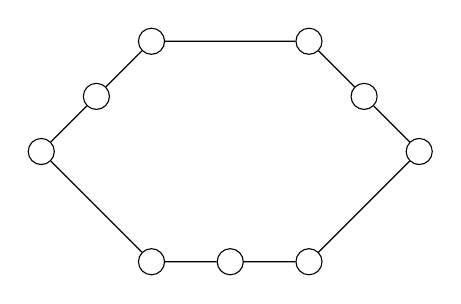
\begin{tikzpicture}
            \node[draw, shape=circle] (1) at (-1,0) {};
            \node[draw, shape=circle] (2) at (0,0) {};
            \node[draw, shape=circle] (3) at (1,0) {};
            \node[draw, shape=circle] (4) at (2.4,1.4) {};
            \node[draw, shape=circle] (5) at (1.7,2.1) {};
            \node[draw, shape=circle] (6) at (1.0,2.8) {};
            \node[draw, shape=circle] (7) at (-1.0,2.8) {};
            \node[draw, shape=circle] (8) at (-1.7,2.1) {};
            \node[draw, shape=circle] (9) at (-2.4,1.4) {};

            \path[draw] (9) -- (1) -- (2) -- (3) -- (4) -- (5) -- (6) -- (7) -- (8) -- (9);
        \end{tikzpicture}
    \end{center}
   
    $P$ tem $\frac{1}{2}(l-1)(k-1)$ pontos sem $k$ pontos em posição estritamente convexa e nem $l$ pontos colineares. Então $q(k,l)>\frac{1}{2}(l-1)(k-1)$, ou seja, $q(k,l)\geq f(k,l)$.

    Se $k$ é par, caso $k=4$, o conjunto de $l-1$ pontos colineares e mais um ponto tem $l$ pontos sem $k$ pontos em posição estritamente convexa. Então $q(4,l)\geq l+1$.
    Caso $k\geq 6$, seja $P$ o conjunto de $(l-1)$ pontos a cada dois lados do $(k-2)$-ágono convexo e mais um ponto que não é colinear com nenhum conjunto de outros dois pontos, como mostrado na figura ($l=4$, $k=6$):
    \begin{center}
        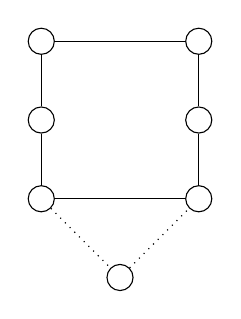
\begin{tikzpicture}
            \node[draw, shape=circle] (2) at (0,0) {};
            \node[draw, shape=circle] (4) at (1.0,1) {};
            \node[draw, shape=circle] (5) at (1.0,2) {};
            \node[draw, shape=circle] (6) at (1.0,3) {};
            \node[draw, shape=circle] (7) at (-1.0,3) {};
            \node[draw, shape=circle] (8) at (-1.0,2) {};
            \node[draw, shape=circle] (9) at (-1.0,1) {};

            \path[draw] (9) -- (4) -- (5) -- (6) -- (7) -- (8) -- (9);
            \path[draw, dotted] (9) -- (2) -- (4);
        \end{tikzpicture}
    \end{center}

    $P$ tem $\frac{1}{2}(l-1)(k-2)+1$ pontos sem $k$ pontos em posição estritamente convexa e nem $l$ pontos colineares. Então $q(k,l)>\frac{1}{2}(l-1)(k-2)+1$, ou seja, $q(k,l)\geq f(k,l)$.

    Agora nós provamos que $q(k,l)\leq f(k,l)$ por indução em $k$ para $k,l\geq 4$.

    Suponha que existam conjuntos com pelo menos $f(k,l)$ pontos sem $k$ pontos em posição extritamente convexa e sem $l$ pontos colineares e seja $P$ um conjunto assim.

    Considere $v_1,v_2,...,v_m$ os vértices de $conv(P)$ nomeados em sentido horário, $v_0 = v_m$ e $v_{m+1}=v_1$. Seja $P_i=\overline{v_iv_{i+1}}\cap P$. Então $2\leq|P_i|\leq l-1$.

    Se $P_i\geq 4$ para algum $P_i$, então $|P\setminus P_i|\geq f(k,l)-(l-1) = f(k-2,l)$. Por indução, $P\setminus P_i$ possui um conjunto $S$ em posição extrietamente convexa com $|S|=k-2$, já que $P$ e, por consequência, $S\subset P$, não possui $l$ pontos colineares. Assim, $S$ com mais dois pontos de $P_i\setminus\{v_i, v_{i+1}\}$ possui $k$ pontos em posição extritamente convexa, o que é uma contradição.

    Então vamos assumir que $P_i\leq 3$ para todo $P_i$.

    Se $P_i = 2$ para algum $P_i$, sejam $t,u,v,w,x,y$ pontos consecutivos de $P$ em sentido horário com $P_i=\{t,w\}$. Como $\{u,v,x,y\}$ estão em posiçã extritamente convexa, $k\geq 5$. Então $|P\setminus\{t,u,v,w,x,y\}|\geq f(k,l)-6 \geq f(k-4,l)$. Por indução, $P\setminus \{t,u,x,w,x,y\}$ possui um conjunto $S$ em posição extritamente convexa com $|S|=k-4$. Então, como $|P_{i-1}|\leq 3$ e $|P_{i+1}|\leq 3$, $S\cup\{u,v,w,x\}$ possui $k$ pontos em posição extritamente convexa, contradizendo a escolha de $P$.

    Então vamos supor que para todo $P_i$, $|P_i|=3$. Assim $|P|=2m$. Seja $S$ o conjunto de um vértice de $P$ a cada dois unido aos pontos de $P$ que não são vértices, como ilustrado na figura com os pontos preenchidos pertencendo a $S$ (se $m$ for ímpar, deixamos dois vértices consecutivos fora de $S$):

    \begin{center}
        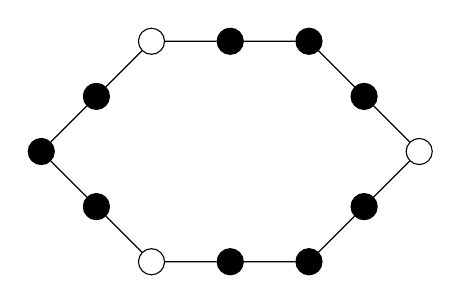
\begin{tikzpicture}
            \node[draw, shape=circle] (1) at (-1,0) {};
            \node[draw, shape=circle, fill] (2) at (0,0) {};
            \node[draw, shape=circle, fill] (3) at (1,0) {};
            \node[draw, shape=circle, fill] (4) at (1.7,0.7) {};
            \node[draw, shape=circle] (5) at (2.4,1.4) {};
            \node[draw, shape=circle, fill] (6) at (1.7,2.1) {};
            \node[draw, shape=circle, fill] (7) at (1.0,2.8) {};
            \node[draw, shape=circle, fill] (8) at (0,2.8) {};
            \node[draw, shape=circle] (9) at (-1.0,2.8) {};
            \node[draw, shape=circle, fill] (10) at (-1.7,2.1) {};
            \node[draw, shape=circle, fill] (11) at (-2.4,1.4) {};
            \node[draw, shape=circle, fill] (12) at (-1.7,0.7) {};

            \path[draw] (12) -- (1) -- (2) -- (3) -- (4) -- (5) -- (6) -- (7) -- (8) -- (9) -- (10) -- (11) -- (12);
        \end{tikzpicture}
        \hspace{2cm}
        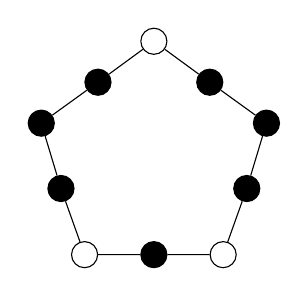
\begin{tikzpicture}
            \node[draw, circle] (1) at (0,1.5) {};
            \node[draw, circle, fill] (2) at (0.71,0.98) {};
            \node[draw, circle, fill] (3) at (1.43,0.46) {};
            \node[draw, circle, fill] (4) at (1.18,-0.37) {};
            \node[draw, circle] (5) at (0.88,-1.21) {};
            \node[draw, circle, fill] (6) at (0,-1.21) {};
            \node[draw, circle] (7) at (-0.88,-1.21) {};
            \node[draw, circle, fill] (8) at (-1.18,-0.37) {};
            \node[draw, circle, fill] (9) at (-1.43,0.46) {};
            \node[draw, circle, fill] (10) at (-0.71,0.98) {};

            \path[draw] (1) -- (2) -- (3) -- (4) -- (5) -- (6) -- (7) -- (8) -- (9) -- (10) -- (1);
        \end{tikzpicture}
    \end{center}
    
    Assim, $S$ está em posição estritamente convexa e $|S|\geq \frac{3|P|-2}{4}=\frac{1}{2}(3m-1)$. Temos que $|P|\geq f(k,l)$ e, como $l\geq 4$, $|P|\geq\frac{3k}{2}-1$. Como $P$ não tem $k$ pontos em posição estritamente convexa, $|S|\leq k-1$. Assim:

    $$8(k-1)\geq 8|S| \geq 12m-4 = 6|P|-4 \geq 9k-10$$

    Isso implica que $k\leq 2$, o que é uma contradição.
\end{proof}

Com isso, podemos generalizar o teorema de Erd\H os-Szekeres como foi feito por \cite{pentagon}.

\begin{teorema}\label{EScolinear}
    Para todo inteiro $k$, todo conjunto com $ES(k)$ pontos contém $k$ pontos em posição convexa (não necessariamente estrita).
\end{teorema}
\begin{proof}
    Sejam $P$ e $P'$ dois conjuntos de pontos no plano com cada ponto de $P$ associado a um único ponto de $P'$. Se para todos $v\in P$ e $v'\in P'$ associados vale que $dist(v,v')<\epsilon$, dizemos que $P'$ é uma $\epsilon$-perturbação de $P$.

    Vamos mostrar o seguinte: para todo conjunto de pontos $P$, existe uma $\epsilon$-perturbação $P'$ de $P$ em posição geral para algum $\epsilon>0$ tal que se $S'$ é um subconjunto de $P'$ em posição estritamente convexa então $S\in P$ (associado a $S'$) está em posição convexa.

    Daí, o teorema de Erd\H os-Szekeres garante que existe para todo $k$ vai existir um $P'$ com $ES(k)$ pontos e $S'\in P'$ em posição estritamente convexa e assim o teorema estará provado.
    
    Para cada tripla ordenada $(u,v,w)$ de pontos de $P$, existe um $\mu>0$ tal que para todo $0<\epsilon<\mu$ toda $\epsilon$-perturbação mantém a orientação\footnote{A orientação de uma tripla ordenada de pontos diz se eles são colineares, se viram para a esquerda ou se para a direita.} desses pontos. Como a quantidade de triplas assim são finitas, pegamos $\mu^*$ o $\mu$ mínimo. Seja $P'$ uma $\mu^*$-perturbação de $P$ em posição geral.

    Seja $S'$ um subconjunto de $P'$ em posição estritamente convexa. Considere $S'$ e sentido horário. Então a orientação de toda tripla de pontos seguidos de $S'$ é para a direita. Como tal perturbação preservou a orientação das triplas não colineares, o conjunto $S$ associado a $S'$ só possuia triplas colineares e orientadas para a direita, quando olhadas da mesma ordem que vimos em $S'$.

    Portanto $S$ está em posição convexa.
\end{proof}
\begin{teorema}
    Dados inteiros $k\geq 3$ e $k\geq 2$, existe um inteiro $\widehat{ES}(k,l)$ tal que todo conjunto $P$ com pelo menos $\widehat{ES}(k,l)$ contém:
    \begin{itemize}
        \item $l$ pontos colineares, ou
        \item $k$ pontos em posição estritamente convexa.
    \end{itemize}
\end{teorema}
\begin{proof}
    Basta mostrar que
    $$
    \widehat{ES}(k,l)\leq
    \begin{cases}
        ES(\frac{1}{2}(k-1)(l-1)+1) \text{ se }k\text{ é ímpar}\\
        ES(\frac{1}{2}(k-2)(l-1)+2) \text{ se }k\text{ é par}
    \end{cases}$$
    Se $k$ é ímpar, seja $P$ um conjunto com $ES(\frac{1}{2}(k-1)(l-1)+1)$ pontos sem $l$ pontos colineares. Pelo teorema \ref{EScolinear}, $P$ possui $\frac{1}{2}(k-1)(l-1)+1$ pontos em posição convexa. Assim, pelo lema \ref{convex}, $P$ possui $k$ pontos em posição estritamente convexa.

    Se $k$ é par, a prova é análoga.
\end{proof}

\subsection{Pentágonos vazios}

Agora que sabemos como achar conjuntos em posição estritamente convexa, vamos mostrar o seguinte teorema de \cite{pentagon}:

\begin{teorema}
    Para todo inteiro $l\geq 2$, todo conjunto finito com pelo menos $ES(\frac{(2l-1)^l-1}{2l-1})$ pontos no plano possui 
    \begin{itemize}
        \item $l$ pontos colineares, ou
        \item um pentágono vazio.
    \end{itemize}
\end{teorema}
\subsubsection {Rascunho da prova}
Considere um conjunto de pontos $P$. A imagem abaixo mostra o que são as camadas convexas de $P$ (formalmente $A_i$ é o conjunto dos vértices de $(P\cap conv(A_{i-1})) \setminus A_{i-1}$).

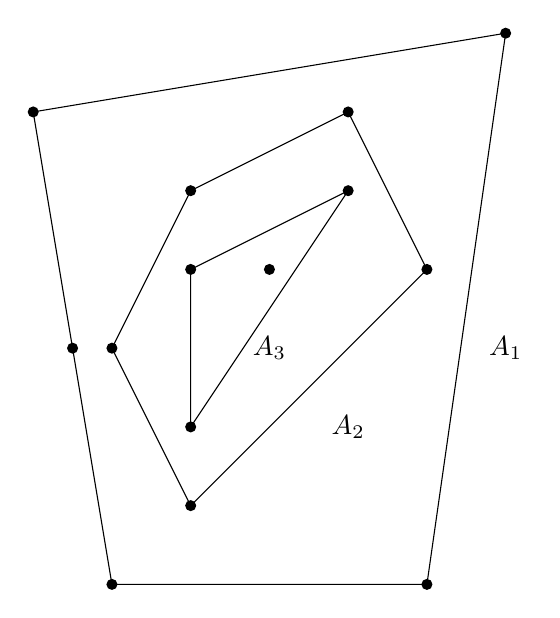
\begin{tikzpicture}
    \foreach \point in {(-0.5,0),(5,4),(-1,3),(3,3),(1,-1),(1,-2),(0,-3),(4,1),(0,0),(4,-3),(3,2),(1,2),(1,1), (2,1)}{
        \fill \point circle (2pt);
    }

    \draw[thin] (5,4) -- (4,-3) -- (4,-3) -- (0,-3) -- (0,-3) -- (-1,3) -- (5,4);
    \draw[thin] (3,3) -- (4,1) -- (1,-2) -- (0,0) -- (1,2) -- (3,3);
    \draw[thin] (1,1) -- (3,2) -- (1,-1) -- (1,1);

    \node(A1) at (5,0) {$A_1$};
    \node(A2) at (3,-1) {$A_2$};
    \node(A3) at (2,0) {$A_3$};
\end{tikzpicture}

Vamos supor que um conjunto suficientemente grande de pontos não tem nenhum pentágono vazio e nem $l$ pontos colineares e achar uma contradição. Para isso, faremos o seguinte:
\begin{enumerate}
    \item Mostrar que tal conjunto tem $l$ camadas convexas não vazias.
    \item Fixar um ponto $z$ que está dentro da $l$-ésima camada convexa.
    \item Mostrar que, para que não tenham pentágonos vazios, muitos pontos têm que se alinhar com $z$ usando um conceito que chamaremos de \textit{arcos vazios}.
\end{enumerate}

\begin{proof}
    Seja $l\geq 3$ e $k=\frac{(2l-1)^l-1}{2l-1}$ e considere um conjunto $P$ com pelo menos $ES(k)$ pontos.

    Suponha que $P$ não contém $l$ pontos colineares nem um pentágono vazio.

    Um conjunto $X\subset P$ em posição convexa com pelo menos $k$ pontos é dito $k$-minimal se não existir outro conjunto $Y\subset P$ em posição convexa com pelo menos $k$ pontos tal que $conv(Y)\subsetneq conv(X)$.

    Pelo teorema \ref{EScolinear}, $P$ possui algum conjunto de $k$ pontos em posição convexa. Seja $A_1$ um conjunto assim $k$-minimal.

    Vamos definir as camadas convexas $A_i$ a partir de $A_1$.
    Para $i\in[l-1]\setminus\{1\}$, seja $A_i$ os vértices de $(P\cap conv(A_{i-1})) \setminus A_{i-1}$ e seja $A_l=(P\cap conv(A_{l-1}))\setminus A_{l-1}$.

    Pelo lema \ref{convex} com $k=5$, para cada $i\in[l-1]\setminus\{1\}$, quaisquer $2l-1$ pontos consecutivos em $A_i$ possuem $5$ pontos em posição estritamente convexa. Para que $P$ não tenha pentágonos vazios, o casco convexo desses $2l-1$ pontos deve conter um ponto de $A_{i-1}$.

    Como $A_{i-1}$ contém $\floor{\frac{|A_{i-1}|}{2l-1}}$ conjuntos distintos de $2l-1$ pontos consecutivos,
    $$|A_i|\geq\floor{\frac{|A_{i-1}|}{2l-1}}>\frac{|A_{i-1}|}{2l-1}-1$$
    E disso concluímos
    $$|A_{i-1}|<(|A_i|+1)(2l-1)$$

    Suponha que para algum $i\in[l-1]$ vale $A_i=\emptyset$. Então $|A_{i-1}| < (2l-1)$, $|A_{i-2}| < (2l-1)^2 + (2l-1)$, $|A_{i-3}| < (2l-1)^3 + (2l-1)^2 + (2l-1)$, ..., e, por indução, 
    $$|A_1|<\sum_{j=1}^{i-1}(2l-1)^j$$
    Somando os elementos da PG, obtemos:
    $$|A_1|=\frac{(2l-1)^i-(2l-1)}{2l-2}<\frac{(2l-1)^i-1}{2l-2}\leq\frac{(2l-1)^l-1}{2l-2}=k$$
    O que é uma contradição. Logo $A_i\neq\emptyset, \forall i \in [l]$. Se $|A_i| < 3$, então $A_{i+1}=\emptyset$. Portanto $|A_i|\geq 3,\forall i \in [l-1]$.

    Fixe $z\in A_l$. Para $i$ em $[l-2]$, considere os pontos de $A_i$ em sentido horário. Se $x$ e $y$ são dois pontos consecutivos nessa ordem, dizemos que o segmento orientado $\overrightarrow{xy}$ é um arco vazio se $\Delta (x,y,z)\cap A_{i+1}=\emptyset$.

    Se $\overrightarrow{xy}$ é um arco vazio em $A_i$, $p$ e $q$ são consecutivos em $A_{i+1}$ em sentido horário e $\overrightarrow{pq}$ é o segmento orientado de $A_{i+1}$ que intercepta com $\Delta(x,y,z)$, então dizemos que $\overrightarrow{pq}$ é o arco seguinte a $\overrightarrow{xy}$.

    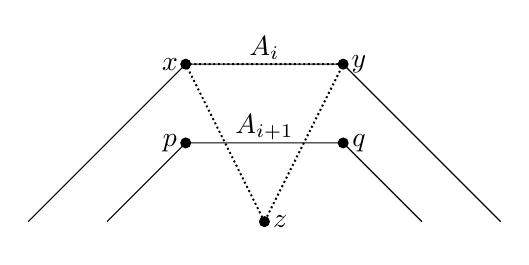
\begin{tikzpicture}
        \foreach \point in {(-1,2),(1,2),(0,0),(-1,1),(1,1)}{
            \fill \point circle (2pt);
        }

        \draw[thin] (-3,0) -- (-1,2) -> (1,2) -- (3,0);
        \draw[thin] (-2,0) -- (-1,1) -- (1,1) -- (2,0);
        \draw[line width=0.25mm, densely dotted] (0,0) -- (-1,2) -- (1,2) -- (0,0);
        \node(Ai) at (0,1.2) {$A_{i+1}$};
        \node(Ai1) at (0,2.2) {$A_i$};
        \node(x) at (-1.2,2) {$x$};
        \node(y) at (1.2,2) {$y$};
        \node(p) at (-1.2,1) {$p$};
        \node(q) at (1.2,1) {$q$};
        \node(z) at (0.2,0) {$z$};
    \end{tikzpicture}

    \begin{fato}\label{fato1}
        Se $\overrightarrow{xy}$ é um arco vazio de $A_i$ e $\overrightarrow{pq}$ é o arco seguinte a $\overrightarrow{xy}$, então $conv(\{x,y,p,q\})$ é um quadrilátero vazio e $\overrightarrow{pq}$ também é um arco vazio.
    \end{fato}
    \begin{proof}
        Seja $Q=\{x,y,p,q\}$. Como $p,q\in conv(A_i)$, $x$ e $y$ são vértices de $Q$ e como $\overrightarrow{xy}$ é um arco vazio $p$ e $q$ também são vértices de $Q$. Logo $Q$ é um quadrilátero. $Q$ é vazio pela definição das camadas convexas.

        Suponha que $\overrightarrow{pq}$ não seja um arco vazio. Então existe algum ponto em $\Delta{p,q,z}\setminus\Delta(x,y,z)$. Seja $t$ um ponto desses mais próximo a $\overline{pq}$. Como $\{x,y,p,q\}$ é um quadrilátero vazio, então $\{x,y,p,q,t\}$ é um pentágono vazio, o que é uma contradição.

        Logo $\overrightarrow{pq}$ é um arco vazio.
    \end{proof}

    Seja $\overrightarrow{pq}$ o arco seguinte ao arco vazio $\overrightarrow{xy}$, então $\overrightarrow{pq}$ é:
    \begin{itemize}
        \item \textbf{alinhado à esqueda} se $p\in\Delta[x,y,z]$ e $q\notin\Delta[x,y,z]$

        \item \textbf{alinhado à direita} se $p\notin\Delta[x,y,z]$ e $q\in\Delta[x,y,z]$
        \item \textbf{alinhado duplamente} se $p\in\Delta[x,y,z]$ e $q\in\Delta[x,y,z]$
    \end{itemize}
    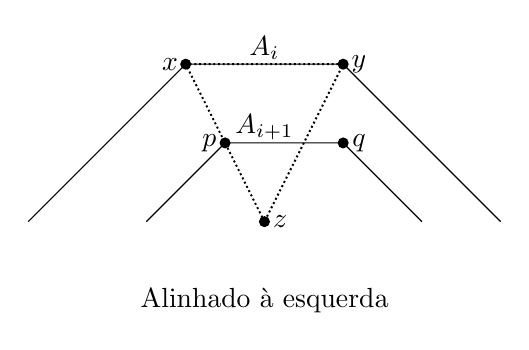
\begin{tikzpicture}
        \foreach \point in {(-1,2),(1,2),(0,0),(-0.5,1),(1,1)}{
            \fill \point circle (2pt);
        }

        \draw[thin] (-3,0) -- (-1,2) -> (1,2) -- (3,0);
        \draw[thin] (-1.5,0) -- (-0.5,1) -- (1,1) -- (2,0);
        \draw[line width=0.25mm, densely dotted] (0,0) -- (-1,2) -- (1,2) -- (0,0);
        \node(Ai) at (0,1.2) {$A_{i+1}$};
        \node(Ai1) at (0,2.2) {$A_i$};
        \node(x) at (-1.2,2) {$x$};
        \node(y) at (1.2,2) {$y$};
        \node(p) at (-0.7,1) {$p$};
        \node(q) at (1.2,1) {$q$};
        \node(z) at (0.2,0) {$z$};
        \node(label) at (0,-1) {Alinhado à esquerda};
    \end{tikzpicture}
    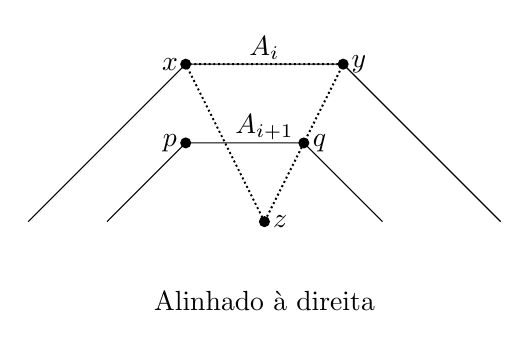
\begin{tikzpicture}
        \foreach \point in {(-1,2),(1,2),(0,0),(-1,1),(0.5,1)}{
            \fill \point circle (2pt);
        }

        \draw[thin] (-3,0) -- (-1,2) -> (1,2) -- (3,0);
        \draw[thin] (-2,0) -- (-1,1) -- (0.5,1) -- (1.5,0);
        \draw[line width=0.25mm, densely dotted] (0,0) -- (-1,2) -- (1,2) -- (0,0);
        \node(Ai) at (0,1.2) {$A_{i+1}$};
        \node(Ai1) at (0,2.2) {$A_i$};
        \node(x) at (-1.2,2) {$x$};
        \node(y) at (1.2,2) {$y$};
        \node(p) at (-1.2,1) {$p$};
        \node(q) at (0.7,1) {$q$};
        \node(z) at (0.2,0) {$z$};
        \node(label) at (0,-1) {Alinhado à direita};
    \end{tikzpicture}
    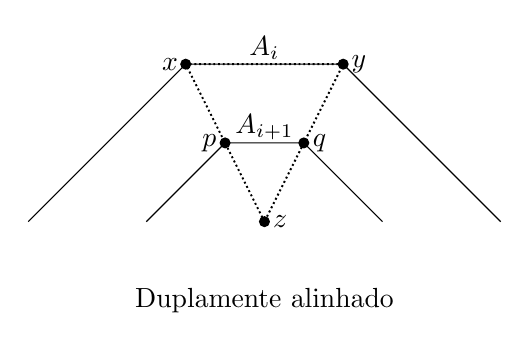
\begin{tikzpicture}
        \foreach \point in {(-1,2),(1,2),(0,0),(-0.5,1),(0.5,1)}{
            \fill \point circle (2pt);
        }

        \draw[thin] (-3,0) -- (-1,2) -> (1,2) -- (3,0);
        \draw[thin] (-1.5,0) -- (-0.5,1) -- (0.5,1) -- (1.5,0);
        \draw[line width=0.25mm, densely dotted] (0,0) -- (-1,2) -- (1,2) -- (0,0);
        \node(Ai) at (0,1.2) {$A_{i+1}$};
        \node(Ai1) at (0,2.2) {$A_i$};
        \node(x) at (-1.2,2) {$x$};
        \node(y) at (1.2,2) {$y$};
        \node(p) at (-0.7,1) {$p$};
        \node(q) at (0.7,1) {$q$};
        \node(z) at (0.2,0) {$z$};
        \node(label) at (0,-1) {Duplamente alinhado};
    \end{tikzpicture}
    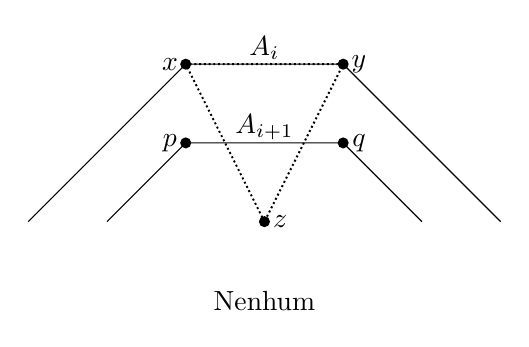
\begin{tikzpicture}
        \foreach \point in {(-1,2),(1,2),(0,0),(-1,1),(1,1)}{
            \fill \point circle (2pt);
        }

        \draw[thin] (-3,0) -- (-1,2) -> (1,2) -- (3,0);
        \draw[thin] (-2,0) -- (-1,1) -- (1,1) -- (2,0);
        \draw[line width=0.25mm, densely dotted] (0,0) -- (-1,2) -- (1,2) -- (0,0);
        \node(Ai) at (0,1.2) {$A_{i+1}$};
        \node(Ai1) at (0,2.2) {$A_i$};
        \node(x) at (-1.2,2) {$x$};
        \node(y) at (1.2,2) {$y$};
        \node(p) at (-1.2,1) {$p$};
        \node(q) at (1.2,1) {$q$};
        \node(z) at (0.2,0) {$z$};
        \node(label) at (0,-1) {Nenhum};
    \end{tikzpicture}

    \begin{fato}\label{fato2}
        Se $\overrightarrow{pq}$ o arco seguinte ao arco vazio $\overrightarrow{xy}$, então $\overrightarrow{pq}$ é alinhado à esquerda ou alinhado à direita ou alinhado duplamente.
    \end{fato}
    \begin{proof}
        Suponha que $\overrightarrow{pq}$ não seja nenhum desses casos.

        Então seja $t$ o ponto em $D=P\cap(\Delta[p,q,z]\setminus\overline{pq})$ mais próximo a $\overline{pq}$. Tal ponto existe pois $z\in D$ e $D$ é finito.

        Como $\overrightarrow{xy}$ é um arco vazio e $\{x,y,p,q\}$ é um quadrilátero vazio, então $\{x,y,p,q,t\}$ é um pentágono vaio, o que é uma contradição.

        Logo $\overrightarrow{pq}$ é alinhado à esquerda ou alinhado à direita ou alinhado duplamente
    \end{proof}
    Suponha que $A_1$ não contenha arcos vazios. Então para dois pontos consecutivos $x$ e $y$ em $A_1$ temos pelo menos um ponto de $A_2$ em $\Delta(x,y,z)$. Como para todos pares de pontos concecutivos $x,y$ e $u,v$ em $A_1$, $\Delta(x,y,z)\cap\Delta(u,v,z)=\emptyset$, teríamos $|A_2|\geq|A_1|$, o que contradiz a minimalidade de $A_1$.

    Seja $\overrightarrow{x_1y_1}$ um arco vazio em $A_1$ e, para $i\in[l-2]$, seja $\overrightarrow{x_{i+1}y_{i+1}}$ o arco seguinte a $\overrightarrow{x_iy_i}$. Pelo fato \ref{fato1}, $\overrightarrow{x_{i+1}y_{i+1}}$ é um arco vazio.

    Se todos os $\overrightarrow{x_iy_i}$ fossem duplamente alinhados, teríamos $\{x_1,x_2,...,x_{l-1},z\}$ colineares e $\{y_1,y_2,...,y_{l-1},z\}$ colineares e, pelo fato \ref{fato2}, $\{x_1,x_2,...,x_{l-1},x_l,z\}$ ou $\{y_1,y_2,...,y_{l-1},y_l,z\}$ seriam colineares, o que é uma contradição.

    Então algum $\overrightarrow{x_iy_i}$ não é duplamente alinhado. Fixe o menor $i\in[l-2]\setminus\{1\}$ que isso acontece. Pelo fato \ref{fato2}, $\overrightarrow{x_iy_i}$ é alinhado à esquerda ou à direita. Sem perda de generalidade, suponha que é alinhado à esquerda. Existe algum $j\in\{i+1,...l-1\}$ tal que $\overrightarrow{x_jy_j}$ não é alinhado à esquerda, pois caso contrário $\{x_1,x_2,...,x_l,z\}$ seriam colineares. Fixe o menor $j\in\{i+1,...,l-1\}$ que isso acontece.

    Temos que $\{x_{j-2},y_{j-2},x_{j-1},y_{j-1},y_j\}$ estão em posição estritamente convexa. Portanto $P$ contém um pentágono vazio.

    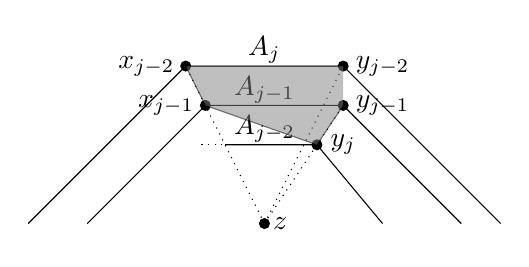
\begin{tikzpicture}
        \foreach \point in {(-1,2),(1,2),(0,0),(0.66666,1),(-0.75,1.5),(1,1.5)}{
            \fill \point circle (2pt);
        }
        \draw[thin] (-3,0) -- (-1,2) -- (1,2) -- (3,0);
        \draw[thin] (-2.25,0) -- (-0.75,1.5) -- (1,1.5) -- (2.5,0);
        \draw[thin] (-0.5,1) -- (0.66666,1) -- (1.5,0);
        \draw[dotted] (-0.8,1) -- (-0.5,1);
        \draw[dotted] (0,0) -- (-1,2);
        \draw[dotted] (0,0) -- (1,2);
        \draw[dotted] (0,0) -- (1,1.5);
        \node(Aj2) at (0,1.2) {$A_{j-2}$};
        \node(Aj1) at (0,1.7) {$A_{j-1}$};
        \node(Aj) at (0,2.2) {$A_j$};
        \node(xj2) at (-1.5,2) {$x_{j-2}$};
        \node(yj2) at (1.5,2) {$y_{j-2}$};
        \node(xj1) at (-1.25,1.5) {$x_{j-1}$};
        \node(yj1) at (1.5,1.5) {$y_{j-1}$};
        \node(yj) at (1,1) {$y_j$};
        \node(z) at (0.2,0) {$z$};
        \draw[opacity=0.5,fill=gray] (1,2) -- (-1,2) -- (-0.75,1.5) -- (0.66666,1) -- (1,1.5);
    \end{tikzpicture}
\end{proof}

Como a melhor cota superior para a ordem de crescimento de $ES(k)$ conhecida é exponencial em $k$ (\cite{ESbound}), esse teorema nos garante a existência de pentágonos vazios em conjuntos de tamanho muito grandes por conter um exponencial duplo.

De fato, \cite{pentagon2} mostraram que o resultado vale para $328l^2$ pontos construindo mais de $l$ camadas convexas com alguma delas com arco vazio e usou o mesmo argumento do teorema a cima.

\begin{corolario}
    A conjectura \ref{conj1} é verdadeira para $k=5$ com $n(5,l)=\Theta(l^2)$.
\end{corolario}
\begin{proof}
    O resultado de \cite{pentagon2} garante que $n(5,l)=O(l^2)$. Para ver que $n(5,l)=\Omega(l^2)$ basta ver que uma grade $(l-1)$x$(l-1)$ contém $(l-1)^2$ pontos e não contém pentágonos vazios nem $l$ pontos colineares.
\end{proof}

\section{Para conjuntos infinitos de pontos}
\cite{infinity} mostraram que a conjectura \ref{conj1} não vale para conjuntos infinitos de pontos com a seguinte construção:

\begin{teorema}
    Existem conjuntos infinitos enumeráveis de pontos sem 4 pontos colineares e sem 3 pontos visíveis dois a dois.
\end{teorema}
\begin{proof}
    Vamos construir indutivamente um conjunto de pontos com tal propriedade.

    Sejam $x_1$, $x_2$ e $x_3$ três pontos não colineares no plano.

    Dados pontos $x_1,...,x_{n-1}$ não conlineares, vamos definir o ponto $x_n$ da seguinte forma: pelo teorema de Sylvester-Gallai, existe uma reta que passa por exatamente dois pontos de $x_1,...,x_{n-1}$. Seja $\mathcal L=\overleftrightarrow{x_ix_j}$ a reta que passa por exatamente dois pontos de $x_1,...,x_{n-1}$ com $i<j$ e com i mínimo entre as com j mínimo. Coloque $x_n$ no segmento $\overline{x_ix_j}$ tal que ela seja a única reta que contenha $x_n$ e mais dois pontos (isso é possível, já que somente uma quantidade finita de pontos de $\mathcal L$ não pode ser escolhida).

    Vamos chamar de $P = \{x_i|i\in \mathbb N\}$. Por construção, $P$ não tem 4 pontos colineares e se $x_i$ e $x_k$ com $i<k$ são visíveis então existe um outro ponto colinear $x_j$ com $j<k$ e $x_k$ está no segmento $\overline{x_ix_j}$.

    Suponha que $x_i$, $x_j$ e $x_k$ são dois a dois visíveis com $i<j<k$. Então existem pontos $x_{i'}$ e $x_{j'}$ com $i'<k$ e $j'<k$ tais que $x_k$ está no segmento $\overline{x_ix_{i'}}$ e no segmento $\overline{x_jx_{j'}}$. Pela escolha de $x_k$, só existe uma reta que contém $x_k$ e mais dois pontos entre $x_1,...x_{k-1}$. Então $i=j'$ e $j=i'$. Mas então $P\cap\overline{x_ix_j}=\{x_i,x_j,x_k\}$, ou seja, $x_i$ e $x_j$ não são visíveis, ou seja, $x_i$ e $x_j$ não são visíveis.

    Portanto não existem 3 pontos visíveis dois a dois em $P$.

\end{proof}

\section{Conclusão}
Embora essa seja uma conjectura com o enunciado relativamente simples, ela é recente e ainda está longe de ser provada. Nos primeiros anos após ser proposta ela recebeu uma atenção considerável entre vários pesquisadores da área, mas não encontramos nada na literatura sobre ela de depois de 2014, o que mostra a dificuldade de se obter qualquer avanço nela atualmente.

Com tamanha dificuldade, Jan Kara propôs o seguinte enfraquecimento da conjectura em uma conversa com Atilla Pór e David R. Wood em 2005, mas também não houve avanços.
\begin{conjectura}
    Dados $k,l\geq 2$, existe um $n=n(k,l)$ tal que todo conjunto finito $P$ com pelo menos $n$ pontos com cada ponto colorido em alguma cor dentre $k-1$ cores ou tem $l$ pontos colineares ou tem um par de pontos da mesma cor visíveis entre si ($\mathcal V(P)$ tem número cromático pelo menos $k$).
\end{conjectura}

Vamos falar de alguns resultados que dificultaram tentativas mais diretas de provar a conjectura e depois vamos falar de algumas áreas que surgiram a partir de outras tentativas de mostrá-la.
\subsection{Dificuldades encontradas}

\subsubsection{Conjuntos de pontos sem heptágonos vazios}
Dado que o teorema de Erd\H os-Szekeres vale, Erd\H os colocou o problema de determinar se para um dado $n$ existe um $g(n)$ tal que todo conjunto com $g(n)$ pontos em posição geral contém um $n$-ágono vazio.

Se essa questão fosse respondida afirmativamente, a conjectura \ref{conj1} sairia como corolário.

Para $n=3$ e $n=4$ é fácil ver que $g(3)=3$ e $g(4)=5$. \cite{Harborth1978} provou que $g(5)=10$ e \cite{Gerken} e \cite{Nicolas} provaram que $g(6)$ existe.

No entanto, \cite{heptagon} mostrou uma construção de conjuntos arbitrariamente grandes sem heptágonos vazios.

\subsubsection{The orchard problem e o grafo de Turán}
\cite{Turan} provou que todo grafo com $n$ vértices e mais arestas que o grafo de Turán $T_{n,k}$\footnote{$T_{n,k}$ é o grafo com $n$ vértices, $k$ cores, dois vértices adjacentes se e somente se têm cores diferentes e a diferença da quantidade de vértices de cada cor no máximo $1$.} tem um subgrafo $K_{n+1}$, então se mostrássemos que todo grafo de visibilidade sem retas com muitos pontos possui muitas arestas conseguiríamos provar a conjectura.

Mas, tentando resolver o \textit{orchard problem}\footnote{Problema do pomar em tradução livre. Dados $n,k$ inteiros, queremos achar o conjunto de $n$ pontos com o máximo de retas que contém $k$ pontos em cada uma delas.}, \cite{Burr1974} e \cite{10.2307/2045427} construiram conjuntos de pontos sem quatro pontos colineares cujo grafo de visibilidade tem menos arestas que o grafo de Turán.

\subsection {Novas direções}

Em 2009, enquato tentava provar a conjectura \ref{conj1}, \cite{blockers} se perguntou quantos pontos são necessário para bloquear a visibilidade de um conjunto de pontos dado. Os resultados obtidos por ele serão vistos no próximo capítulo, mas a partir disso surgiram várias outras questões sobre visibilidade de pontos e bloqueadores de visibilidade.

